\documentclass[screen, aspectratio=43]{beamer}
\usepackage[T1]{fontenc}
\usepackage[utf8]{inputenc}

% Use the NTNU-temaet for beamer 
% \usetheme[style=ntnu|simple|vertical|horizontal, 
%     language=bm|nn|en, 
%     smalltitle, 
%     city=all|trondheim|alesund|gjovik]{ntnu2017}
\usetheme[style=ntnu,language=en]{ntnu2017}

\usepackage[english]{babel}
\usepackage[style=numeric,backend=biber,natbib=false,sorting=none]{biblatex}

\title[PCW-d1]{Physical Computing Workshop}
\subtitle{Introduction}
\author[A. Xamb{\'o}]{Anna Xamb{\'o}}
\institute[NTNU]{Department of Music, NTNU}
%\date{16 October 2018}
%\date{} % To have an empty date

\addbibresource{../pcw.bib} % Add bibliography database

% Set the reference style to numeric.
% See here: http://tex.stackexchange.com/questions/68080/beamer-bibliography-icon
\setbeamertemplate{bibliography item}[text] 

% Set bibliography fonts to a small size.
\renewcommand*{\bibfont}{\footnotesize}

\begin{document}

\begin{frame}
  \titlepage
\end{frame}

% Alternatively, special title page command to get a different background
% \ntnutitlepage

\begin{frame}
\frametitle{Workshop Design Criteria}
\begin{itemize}
\item Facilitate a hands-on workshop with available, low-tech technology (e.g. mobile phones, contact mics, arduinos, web audio).
\item Explore individually and in group the fundamental concepts behind physical computing (e.g. tinkering, programming, making).
\item Promote a sharing culture of code and discoveries (e.g. writing reflective blogposts, sharing the code on github).
\item Contextualize the workshop to the broader context of interactive systems for music performance at both theoretical and practical levels (e.g. readings, concerts).
\end{itemize}
\end{frame}
%
\begin{frame}
\frametitle{What is the Workshop About?}
\begin{itemize}
\item An intense 4-day workshop where you will explore physical computing and interactive systems.
\item For the first three days, there will be a theme with paced exercises.
\item At the beginning of each session there will be a warm-up discussion based on a relevant related reading.
\item At the end of each session there will be a network music performance to showcase the own-built prototype.
\item Each team will write a blog post about the challenges and opportunities of their own-built prototype.
\item On the last day, there will be a mini-hackathon where you will develop an interactive system for music performance mixing technologies and techniques learned throughout the workshop.
\end{itemize}
\end{frame}
%
\begin{frame}
\frametitle{Schedule Diagram}
\begin{figure}
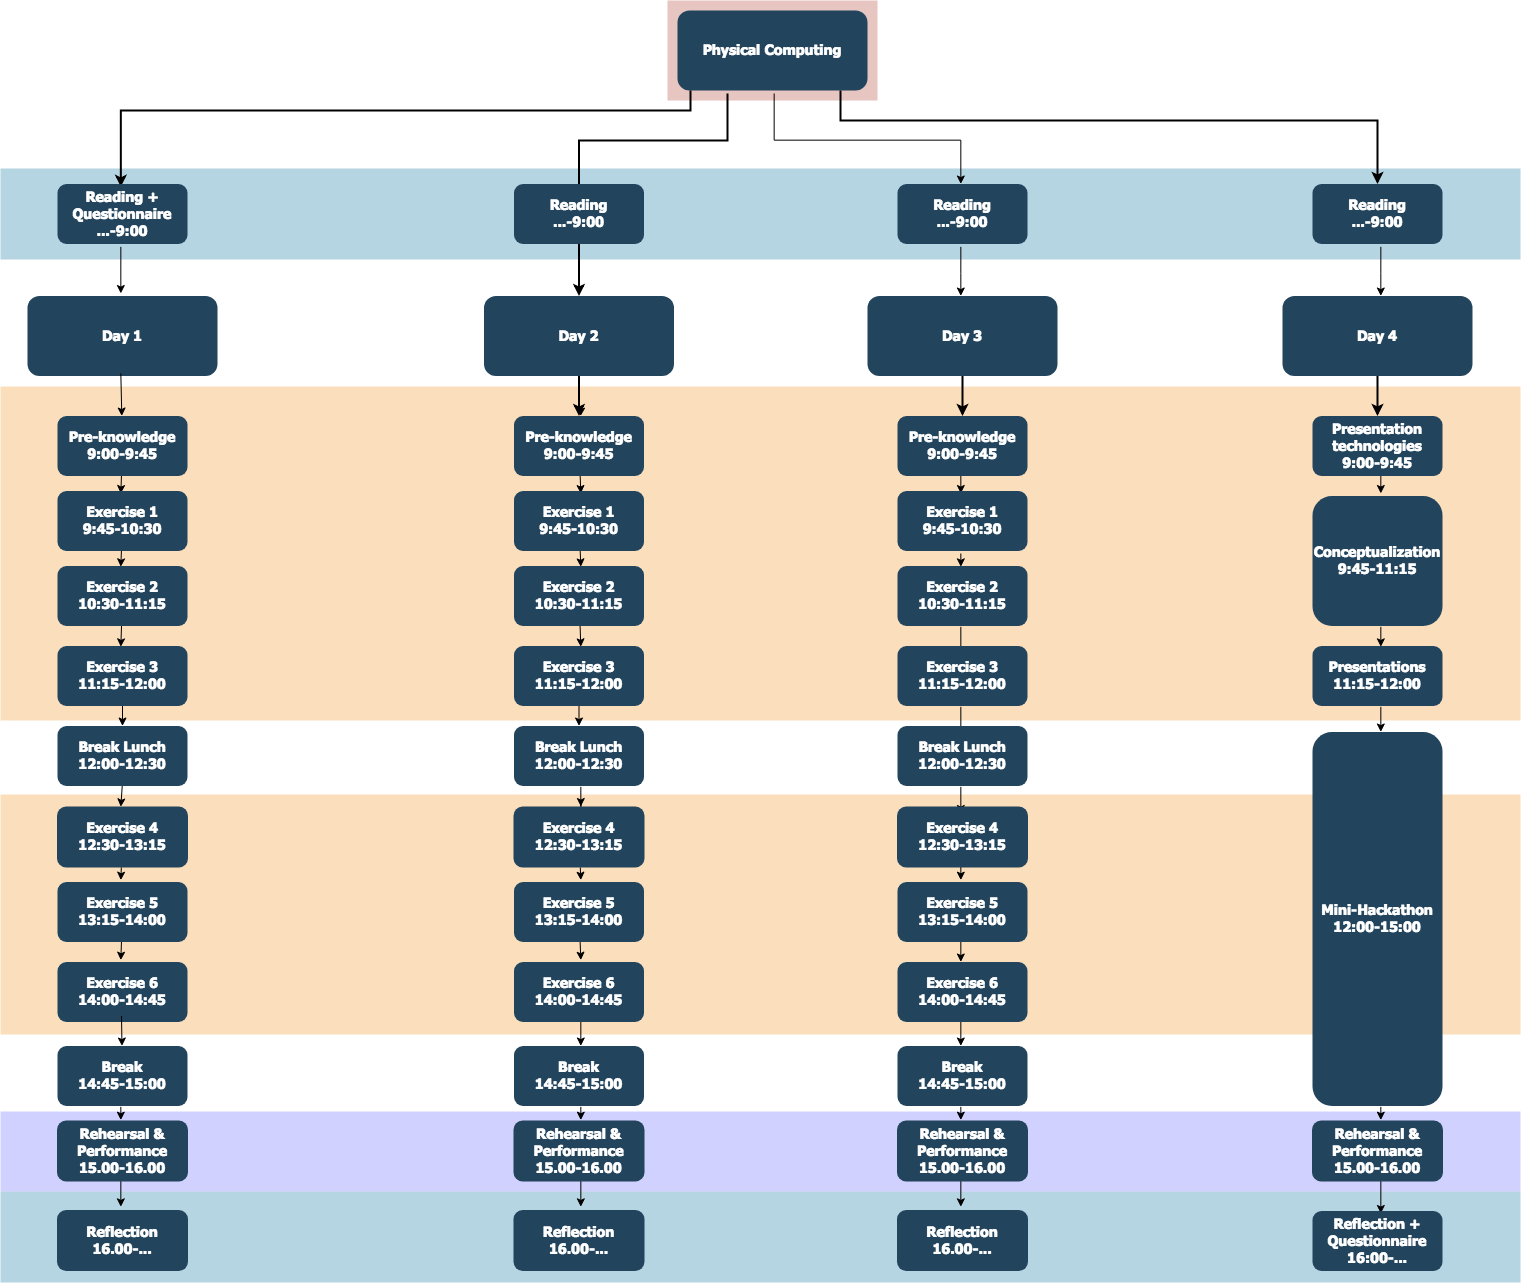
\includegraphics[scale=0.17]{img/Outline-PC-workshop.png}
\end{figure}
\end{frame}
%
\begin{frame}
\frametitle{General Learning Outcomes}
\begin{itemize}
\item Develop skills of computational thinking and programming.
\item Explore how to create a prototype of an interactive system for music performance with low-tech technologies.
\item Discover iterative design and the possibilities of network music by performing with own-built prototypes.
\item Develop critical thinking skills applied to reflection on artistic practice and instrument building.
\end{itemize}
\end{frame}
%
\begin{frame}
\frametitle{General Approach}
\begin{itemize}
\item This workshop should be seen a starting point to get interest with physical computing applied to music tech.
\item It has been designed to be low tech, that is, using open source or consumer affordable gadgets, except for the last day.
\item Daily attendance is expected, as well as the completion of assignments before and after class.
\end{itemize}
\end{frame}
%
\begin{frame}
\frametitle{What it is not}
\begin{itemize}
\item An in-depth tutorial of a particular technology.
\item A technical course: just enough to build things!
\item A course about soldering.
\end{itemize}
However... related resources will be provided.
\end{frame}
%
\begin{frame}
\frametitle{Grading}
\begin{itemize}
\item 40\% Individual work\\
\emph{You need to participate in the discussion/quizzes about the readings and document your personal contributions in the code to get a positive grade.}
\item 40\% Group work\\
\emph{You will be expected to participate in the daily performance and blogpost to have a positive grade.}
\item 20\% Participatory assistance\\
\emph{An overall participatory attitude and regular assistance can improve the grade.}
\end{itemize}
\end{frame}
%
\begin{frame}
\frametitle{Previous Knowledge / Preparation}
\begin{itemize}
\item Every day you should check if there is a list of items that need to be brought to class.
\item Every day you should check the suggested reading that will be discussed at the beginning of the class.
\item It is not required, but if interested, you can start looking at the following hardware and web technologies: Handwaving.js, Arduino, P5.js, Tone.js, Flocking.js, LittleBits. 
\item For the mini-hackathon, you are allowed to bring / explore other technologies of your interest e.g. Myo bracelets, Bela platform, and so on.
\end{itemize}
\end{frame}
%
\begin{frame}
\frametitle{Recommended General Readings}
\begin{figure}
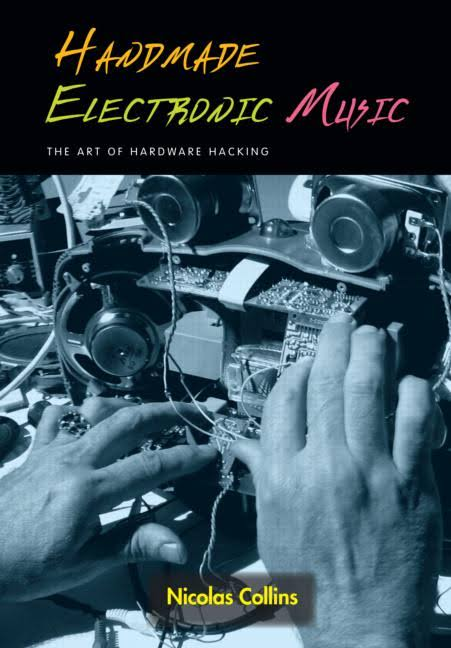
\includegraphics[scale=0.14]{img/HEM-collins-book.jpg}
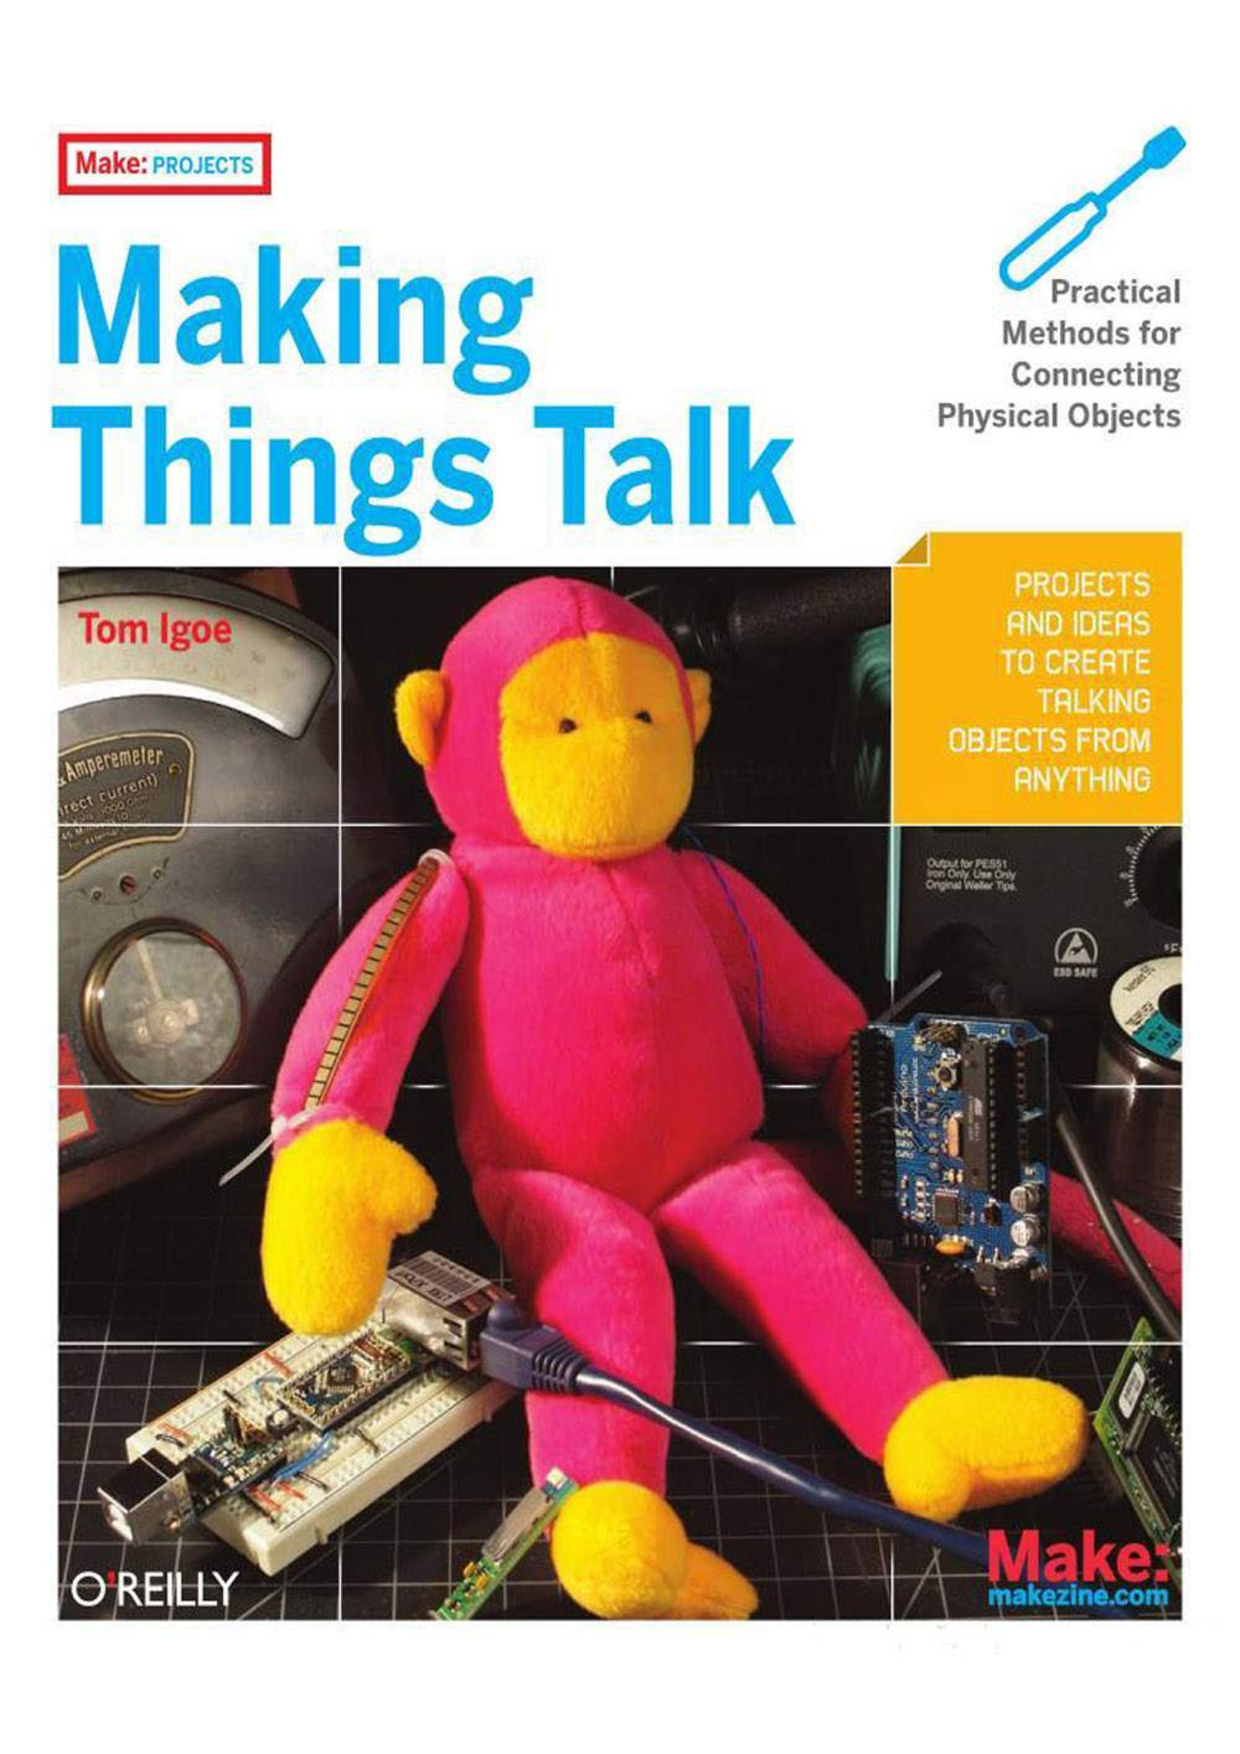
\includegraphics[scale=0.12]{img/makingthingstalk.pdf}
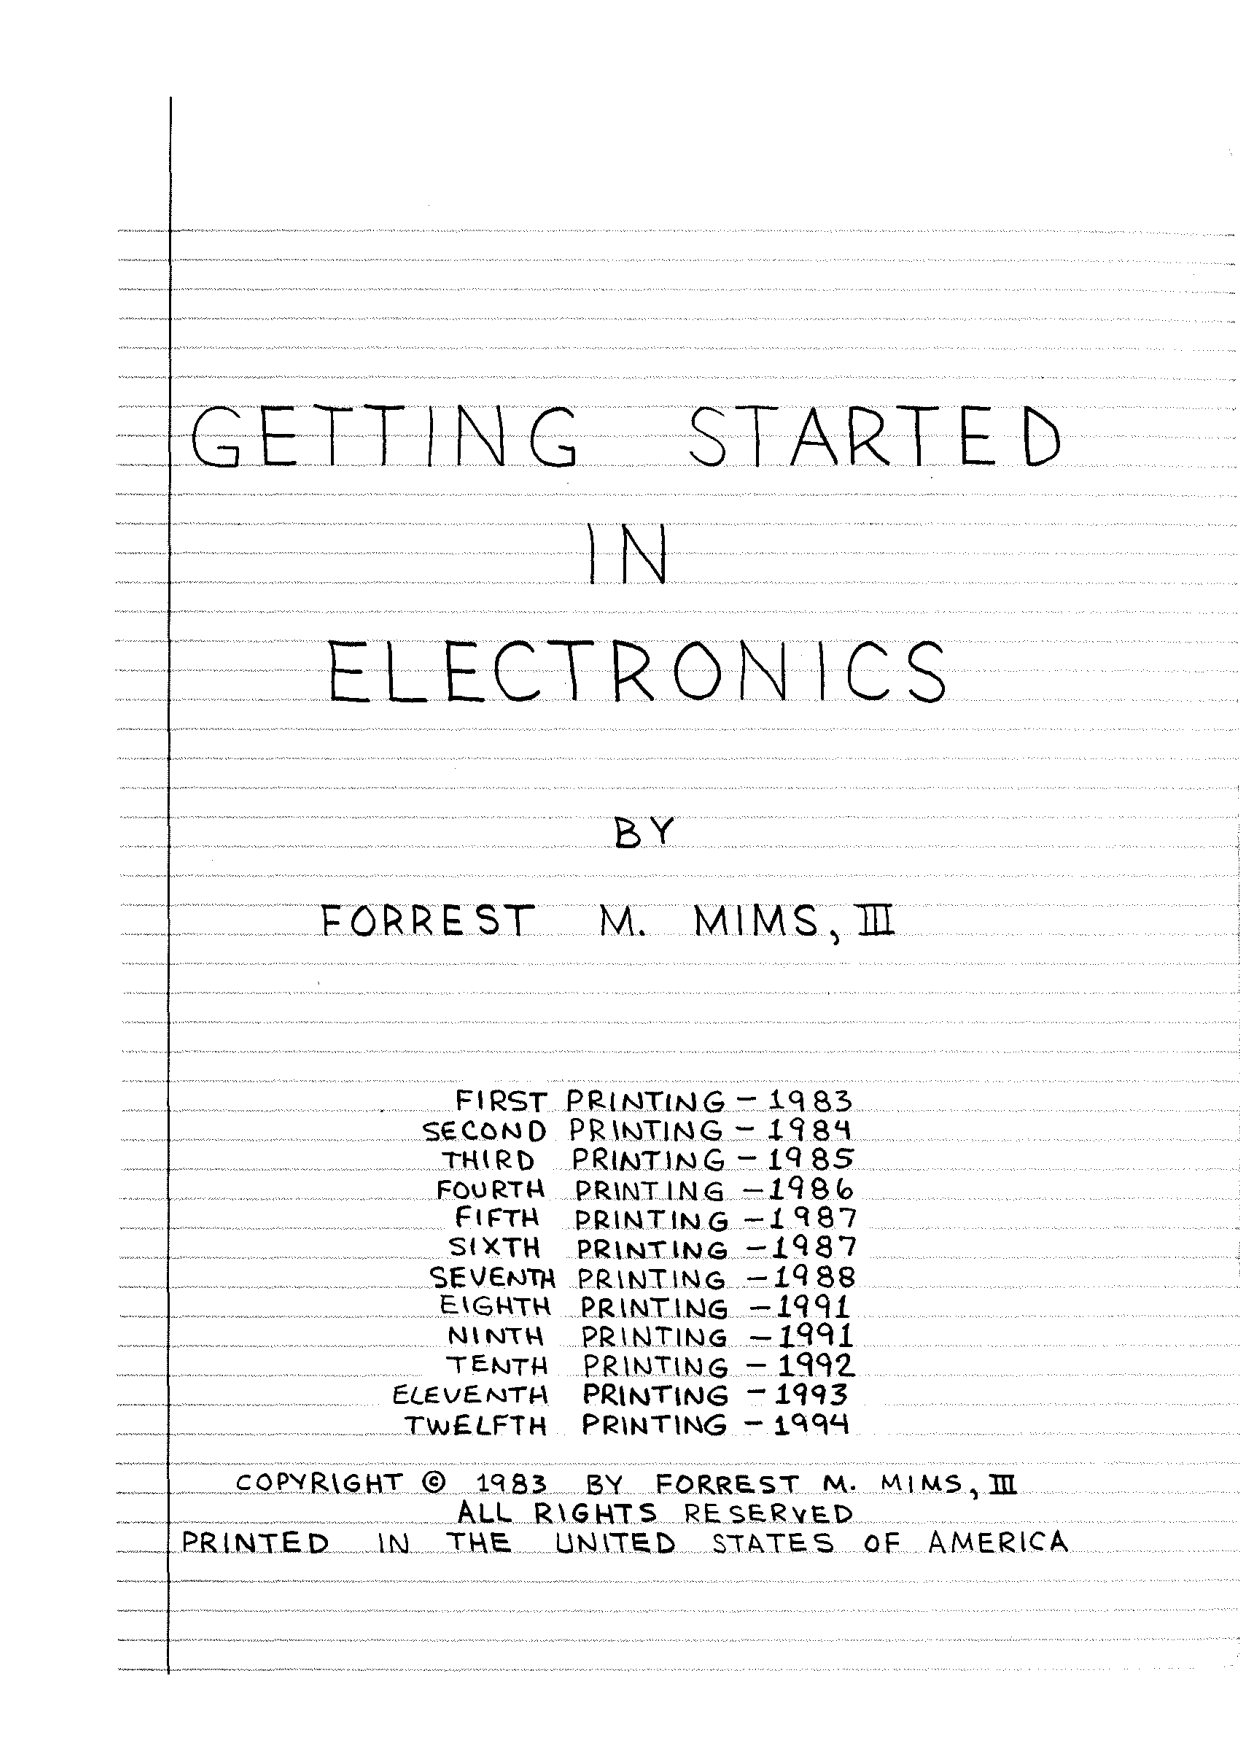
\includegraphics[scale=0.12]{img/gettingstartedelectronics-book.pdf}
\end{figure}
\begin{itemize}
\item The book \emph{Handmade Electronic Music} by Nicolas Collins~\cite{Collins.2006.handmadebook}.
\item ... and in general all the videos related to Collins' book:\\
\url{https://www.nicolascollins.com/video/}
\item The book \emph{Making Things Talk} by Tom Igoe~\cite{Igoe.2007.making}.
\item The book \emph{Getting Started in Electronics} by Forrest Mims~\cite{Mims.1983.radioshack}.
\end{itemize}
\end{frame}
%
\begin{frame}
  \frametitle{References}
  \printbibliography
\end{frame}
%
\end{document}
